\documentclass{article}
\usepackage[margin=1.0in]{geometry}
\usepackage{hyperref}
\usepackage{amsmath}
\usepackage{amsfonts}
\usepackage{tikz}
\title{Approximating Imperative Programs as Neural Networks for Automated Correction}
\author{Andrew Bruce \\ \href{mailto:acbruce@ucsc.edu}{acbruce@ucsc.edu}
  \and Dongjing Wang \\ \href{mailto:dwang114@ucsc.edu}{dwang114@ucsc.edu}
  \and Ming Qi \\ \href{mailto:mqi6@ucsc.edu}{mqi6@ucsc.edu} }

\begin{document}
\maketitle
\section*{Motivation}
We aim to approximate gradient descent on discrete code. When software engineers write tests for their code, these tests can act as a loss function.
\section*{Theory and Implementation}
This draft of a textbook \cite{blondel2024elementsdifferentiableprogramming} released during summer 2024 provides the background for approximating program data structure operations and control flow as differentiable functions, similar to a neural network.\\
An example is if $\vec{l} \in \mathbb{R}^{n_{\ge 1}}$ is a list and there is some discrete function such as $max$:
\begin{center}
  $\mathrm{max} \in \mathbb{R}^{n_{\ge 1}} \rightarrow \mathbb{R}$\\
  $\mathrm{max}(\vec{l}) = l_{\mathrm{max}}$
\end{center}
But when attempting to differentiate
\begin{center}
  $$\dfrac{d \mathrm{max}(\vec{l})}{dl_i} = \left\{
  \begin{array}{ll}
    1 & l_i = l_{\mathrm{max}} \\
    0 & \mathrm{otherwise}
  \end{array} 
  \right.$$
\end{center}
Giving null derivatives when changing components of the list that are not the current maximum element.
One can define a ``soft'' approximation of these discrete functions from a stochastic point of view, usually having the advantage of differentiability.
\begin{center}
  $\mathrm{max} \approx \mathrm{softmax}$\\
  $\mathrm{softmax} \in \mathbb{R}^n \rightarrow \mathbb{R}^n$\\
  $\mathrm{softmax}(\vec{l})_i = \dfrac{e^{\vec{l}_i}}{\sum_{j=1}^n e^{\vec{l}_j}}$\\
\end{center}
This can be generalized to other programming concepts such as logical comparisons, data structures, and control flow.
\begin{center}
  \begin{tabular}{ |c|c| }
    \hline
    normal & soft variant \\
    \hline
    $(\ge) = \mathrm{ge} \in (\mathbb{R} \times \mathbb{R}) \rightarrow \{ 0, 1 \}$ & $\mathrm{softge} \in (\mathbb{R} \times \mathbb{R}) \rightarrow [ 0, 1 ]$\\
    $(=) = \mathrm{eq} \in (\mathbb{R} \times \mathbb{R}) \rightarrow \{ 0, 1 \}$ & $\mathrm{softeq} \in (\mathbb{R} \times \mathbb{R}) \rightarrow [ 0, 1 ]$\\
    $\mathrm{ifelse} \in (\{ 0, 1 \} \times F \times F) \rightarrow F$ & $\mathrm{softifelse} \in ([ 0, 1 ] \times F \times F) \rightarrow F$\\
    $\mathrm{listget} \in (\mathbb{R}^n \times [n] ) \rightarrow \mathbb{R}$ & $\mathrm{softlistget} \in (\mathbb{R}^n \times \Delta^n ) \rightarrow \mathbb{R}$\\
    $\mathrm{listset} \in (\mathbb{R}^n \times \mathbb{R} \times [n] ) \rightarrow \mathbb{R}^n$ & $\mathrm{softlistset} \in (\mathbb{R}^n \times \mathbb{R} \times \Delta^n ) \rightarrow \mathbb{R}^n$\\
    $\mathrm{listinsert} \in (\mathbb{R}^n \times \mathbb{R} \times [n+1] ) \rightarrow \mathbb{R}^{n+1}$ & $\mathrm{softlistinsert} \in (\mathbb{R}^n \times \mathbb{R} \times \Delta^{n+1} ) \rightarrow \mathbb{R}^{n+1}$\\
    \hline
  \end{tabular}
\end{center}
Once a program is differentiable and without null derivatives it can be treated just like a neural net. Deep learning techniques such as backpropagation and gradient descent can be applied to programs. We would have to manually write a the gradient calculation, backpropagation and Newton's method. Possibly by leveraging NumPy's automatic differentiation capabilities
\section*{Example}
A very simple and non-practical example:
\begin{verbatim}
bool is_greater_than_2(double num){
  if(num > 3.0){
    return true;
  }else{
    retun false;
  }
}
\end{verbatim}
The code is trivially incorrect. After transforming it into a soft variant, and some test cases it could look like:
\begin{verbatim}
double is_greater_than_2(double num){
  return softifelse(softgt(num, 3.0), 1.0, 0.0);
}

void test_case_1(){
  assert(is_greater_than_2(3) == 1.0);
}
void test_case_2(){
  assert(is_greater_than_2(2) == 0.0);
}
void test_case_3(){
  assert(is_greater_than_2(1.9) == 0.0);
}
void test_case_4(){
  assert(is_greater_than_2(-2) == 0.0);
}
\end{verbatim}
In the above example the code is incorrect because it is testing if it is greater than 3, rather than 2. We can represent the code as a neural net like:\\
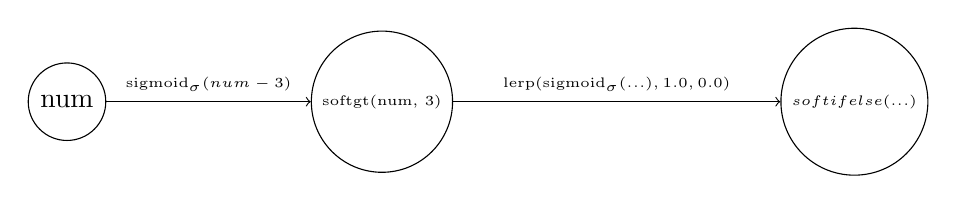
\begin{tikzpicture}[main/.style = {draw, circle}] 
  \node[main] (1) {num};
  \node[main] at (0:4cm) (2)  {\tiny softgt(num, 3)}; 
  \draw[->] (1) -- node[above]{\tiny $\text{sigmoid}_{\sigma}(num-3)$} (2);
  \node[main] at (0:10cm) (3)  {\tiny $softifelse(...)$};
  \draw[->] (2) -- node[above]{\tiny $\text{lerp}(\text{sigmoid}_{\sigma}(...), 1.0, 0.0)$} (3);
\end{tikzpicture}
Then, for example the 3 (and more) can be replaced by a parameter $C$ which can be trained on using gradient descent, with the loss function specified by the hand written test cases.
\begin{center}
  $C_0 = 3, C_{N+1} = C_{n} - \lambda \nabla_C L(C, ...)$
\end{center}
This transformation should be applicable to any programs that we can formulat a ``soft'' transformation for, such as sorting algorithms. Fixed length for loops can be unrolled, and while loops can be represented with a possibly infinitely long Markov chain.
\section*{Previous work}
One such previous work is ``Zygote'' \cite{DBLP:journals/corr/abs-1907-07587}, a framework for differentiating Julia programs. Another example includes a purely function IR language called ``Myia'' \cite{DBLP:journals/corr/abs-1810-11530}. Both of these have not been used for program correction, and do not support more complex control flows such as list or dictionary operations such as getting and setting. These works seem to focus on an exact differentiation rather than a possibly more usefull approximation. It prevents using discrete operations or discontinous functions causing null derivatives as part of the gradient, preventing gradient descent from optimizing that parameter any further. These both are also used to back propigate from the inputs of the program, but not differentiate with respect to the program parameters itself. They have not been applied with backpropagation for for automatic code correction.
\section*{Novelty}
As far as We know no one has implemented this approach before.
\section*{Synthetic Data Generation}
The general algorithm would take in data in the form of test cases for a function for each instance of a learning problem. We will have to manually write programs and test cases for each program to see if the algorithm converges on the correct answer. Test cases can be trivially generated from the correct algorithm. We can also generate instances of the learning problem by automatially changing the parameters of a correct program to be incorrect, such as a wrong offset on a list index. Each instance can test if the backpropagation and gradient descent will converge on the correct algorithm.
\section*{Limitation}
Have not verified that you can take the second derivative, the Hessian, for the second order Newton's method $x_{\mathrm{new}} = x_{\mathrm{old}} - [\nabla^2 f]^{-1}(x) \nabla f(x)$.\\
The gradient is applied on the approximation of a program, not the actual program. When the loss of the approximation converges to zero, it does not necessarily mean that the real program will become correct.
\bibliographystyle{abbrv}
\bibliography{refs}
\end{document}
